\documentclass[compress]{beamer}

% fonts p14; 18.2.3
% Futura font

% Cambridge, Copenhagen, JuanLesPins, Luebeck, Malmoe, Marburg,
% Montpellier, PaloAlto, Singapore

% colortheme beaver, dolphin

% Copyright 2004 by Till Tantau <tantau@users.sourceforge.net>.
%
% In principle, this file can be redistributed and/or modified under
% the terms of the GNU Public License, version 2.
%
% However, this file is supposed to be a template to be modified
% for your own needs. For this reason, if you use this file as a
% template and not specifically distribute it as part of a another
% package/program, I grant the extra permission to freely copy and
% modify this file as you see fit and even to delete this copyright
% notice. 

\mode<presentation> {
  \usetheme{Malmoe}
  \usecolortheme{beaver}
  \setbeamercovered{transparent}
  \setbeamertemplate{navigation symbols}{}
  \setbeamertemplate{footline}{%
    \leavevmode%
    \hbox{\begin{beamercolorbox}[wd=\paperwidth,ht=0.5ex,dp=1.125ex,leftskip=.3cm,rightskip=.3cm plus1fil]{title in head/foot}%
    \end{beamercolorbox}}%
    \vskip0pt%
  }
}

\usepackage[english]{babel}
\usepackage[latin1]{inputenc}
\usepackage{helvet}
\usepackage{xspace}
% Or whatever. Note that the encoding and the font should match. If T1
% does not look nice, try deleting the line with the fontenc.
%\usepackage[T1]{fontenc}
\usepackage[normalem]{ulem}
\usepackage{calc}
\usepackage{verbatim}
\usepackage{multirow}
\usepackage{dcolumn}

\graphicspath{{figs-slides/}{figs-techreport/}}

\newcommand{\an}{\emph{Astrometry.net}\xspace}
\newcommand{\libkd}{\emph{libkd}\xspace}
\newcommand{\kdtree}{$kd$-tree}
\newcommand{\antoc}{Astrometry.net\xspace}
\newcommand{\eg}{\emph{eg}}

\newcommand{\commentout}[1]{}

\title[\an]
{\an: automatic recognition and calibration of astronomical images}
  
%\newcommand{\fancy}{\hspace{0.5em}--\hspace{0.5em}}
\newcommand{\fancy}{\hspace{1.5em}}
%\author[Lang -- Roweis -- Hogg]{\fancy Dustin~Lang \fancy Sam~Roweis \fancy David~W.~Hogg \fancy }
\author{Dustin Lang}

\date{2009-09-10}

\subject{x}

% If you have a file called "university-logo-filename.xxx", where xxx
% is a graphic format that can be processed by latex or pdflatex,
% resp., then you can add a logo as follows:
% \pgfdeclareimage[height=0.5cm]{university-logo}{university-logo-filename}
% \logo{\pgfuseimage{university-logo}}

\begin{document}

\begin{frame}
  \titlepage
\end{frame}

\section{Goal}

\subsection{The goal}

\begin{frame}[fragile]{The goal: recognition of astronomical images}
  \vspace{-1ex}
  \only<1>{You give us an astronomical image}
  \only<2>{We tell you where your telescope was pointing \\ \hspace{12pt}{\small location, scale, and rotation---World Coordinate System (WCS)}}
  \only<3>{\ldots and tell you what's in your image}
  \\
  \only<1>{\includegraphics[height=0.9\textheight]{pleiades}}
  \only<3>{\includegraphics[height=0.9\textheight]{pleiades_ann}}
   \only<2>{%
    \includegraphics[width=0.32\textwidth]{pleiades_zoom_1}
    \hspace{0.2ex}%
    \includegraphics[width=0.32\textwidth]{pleiades_zoom_2}
    \hspace{0.2ex}%
    \includegraphics[width=0.32\textwidth]{pleiades_zoom_3}
   }
   \\
   \only<2>{\begin{tiny}
\verbatiminput{pleiades.txtwcs}
\end{tiny}}
  \vfill
\end{frame}

\section{Approach}

\subsection{Outline}

\begin{frame}{\an: The approach: geometric hashing}
  \begin{itemize}
    \addtolength{\itemsep}{0.5ex}
  \item Match \alert{features} in the image to features in an \alert{index}
    \begin{itemize}
    \addtolength{\itemsep}{0.5ex}
    \item Features are based on the \alert{geometric arrangement} of small groups of stars
    \item The \alert{index} maps \alert{features} to \alert{places on the sky}
    \end{itemize}
  \item Each feature match is a \alert{hypothesis} about the alignment of the image on the sky
  \item \alert{Verify} the hypotheses to reject false matches
  \end{itemize}
\end{frame}

\begin{frame}{\an: The geometric feature}
  \begin{columns}
	\begin{column}{0.5\textwidth}
	  \begin{center}
		\makebox[0.5\textwidth][c]{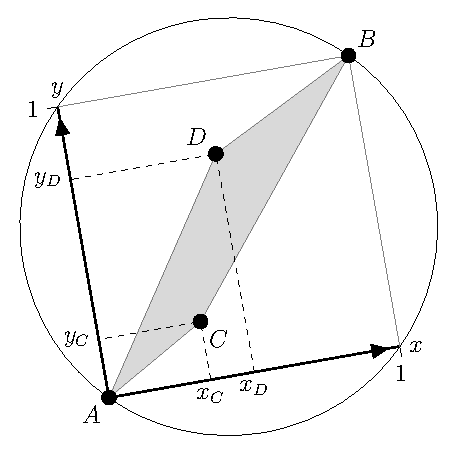
\includegraphics[width=1.2\textwidth]{quad-fig}}
	  \end{center}
	\end{column}
	\begin{column}{0.5\textwidth}
	  \begin{itemize}
      \item Four-star features
	  \item Two \alert{most distant} stars are labelled $A$, $B$
	  \item They establish a \alert{local coordinate frame}
	  \item Two others stars are labelled $C$ and $D$
	  \item Their positions in the local coordinate frame become the
		\alert{feature descriptor}, $(C_x, C_y, D_x, D_y)$
      \item Has the \alert{invariances} we need: translation, scale, and rotation
	  \end{itemize}
	\end{column}
  \end{columns}
\end{frame}


\subsection{Indexing}

\begin{frame}{\an: Indexing}
  \begin{itemize}
  \item Stars in the USNO-B reference catalog are distributed
    \alert{non-uniformly}
  \item We want to be able to recognize images anywhere on the sky equally well:
	Need to \alert{uniformize}.
  \end{itemize}

  \begin{center}
	
\includegraphics[height=0.6\textheight]{usnob-density}
  \end{center}
\end{frame}


\newlength{\cwone}
\setlength{\cwone}{0.7\textwidth}
\newlength{\cwtwo}
\setlength{\cwtwo}{0.3\textwidth}
\newlength{\indfigh}
\setlength{\indfigh}{0.94\textheight}
\begin{frame}[plain]{\an: Indexing}
  \setlength{\leftmargin}{0pt}
  \begin{columns}[onlytextwidth]
	\column{\cwone}
    \hspace{-10pt}
	\setlength{\fboxsep}{0pt}
	\makebox[\cwone][r]{%
	  \fbox{%
		\only<1>{\includegraphics[height=\indfigh]{usnob}}%
		\only<2>{\includegraphics[height=\indfigh]{usnob-grid}}%
		\only<3>{\includegraphics[height=\indfigh]{cut2}}%
		\only<4>{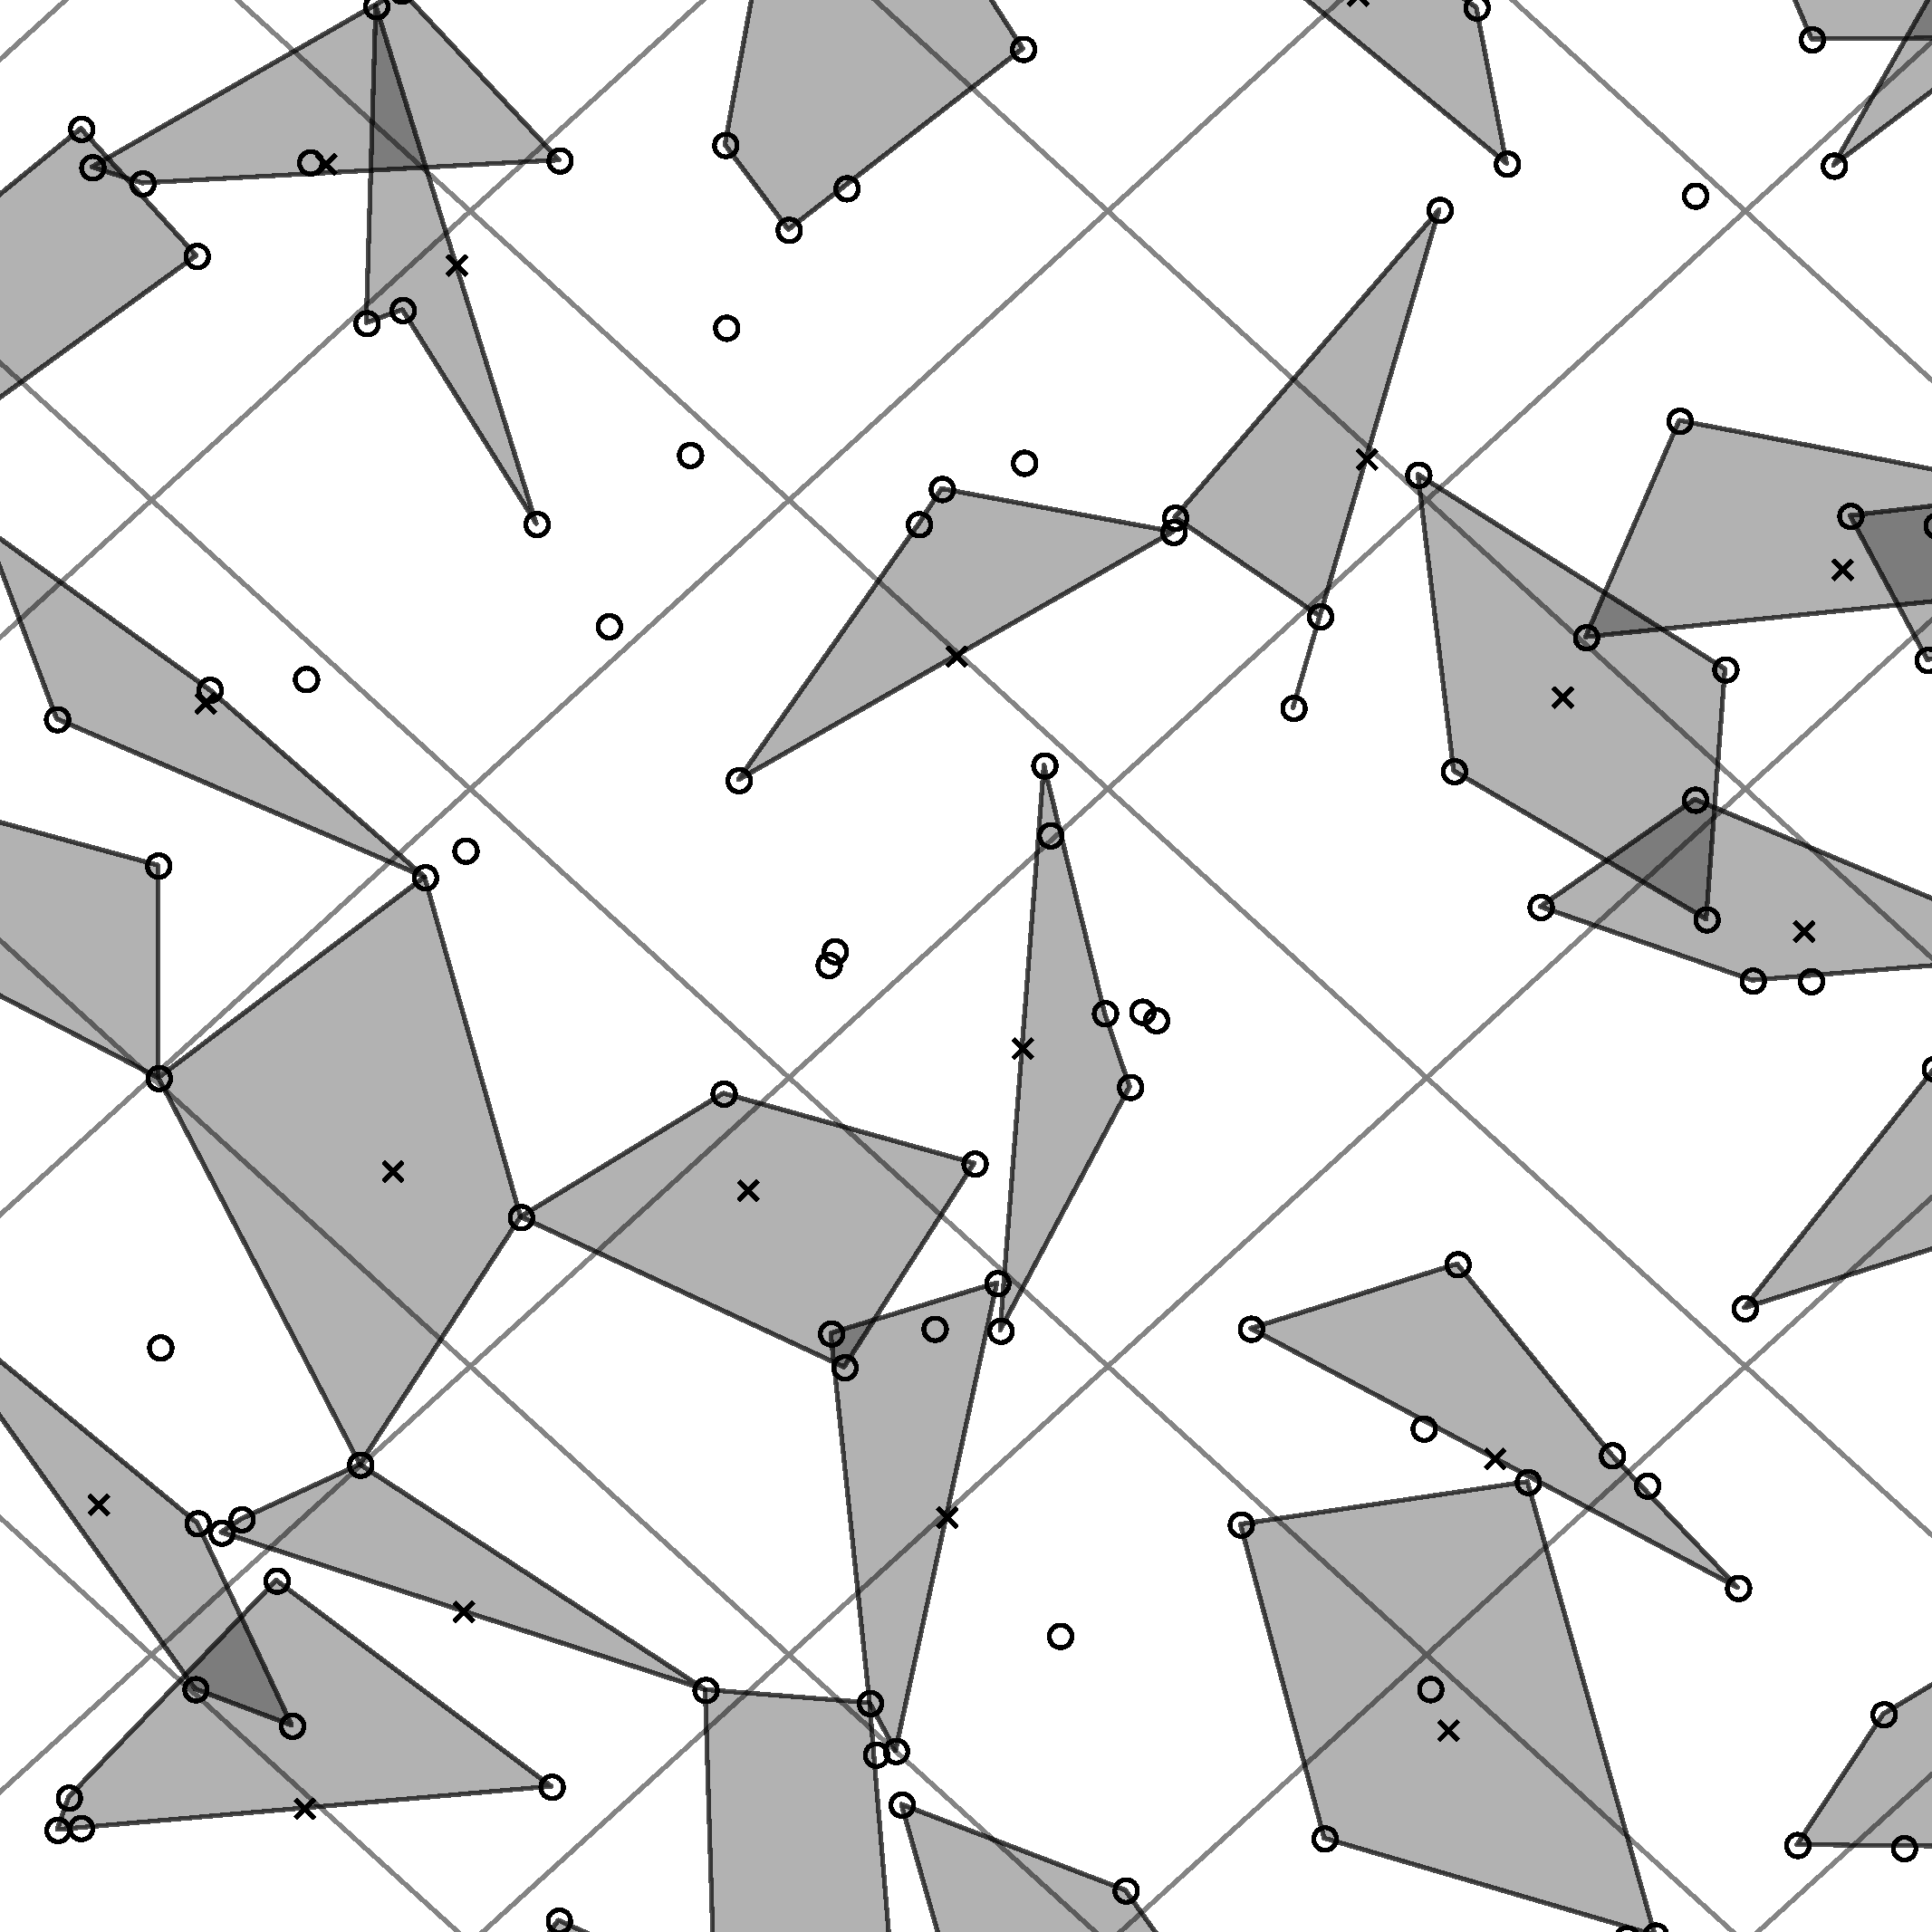
\includegraphics[height=\indfigh]{quads1b}}%
		\only<5>{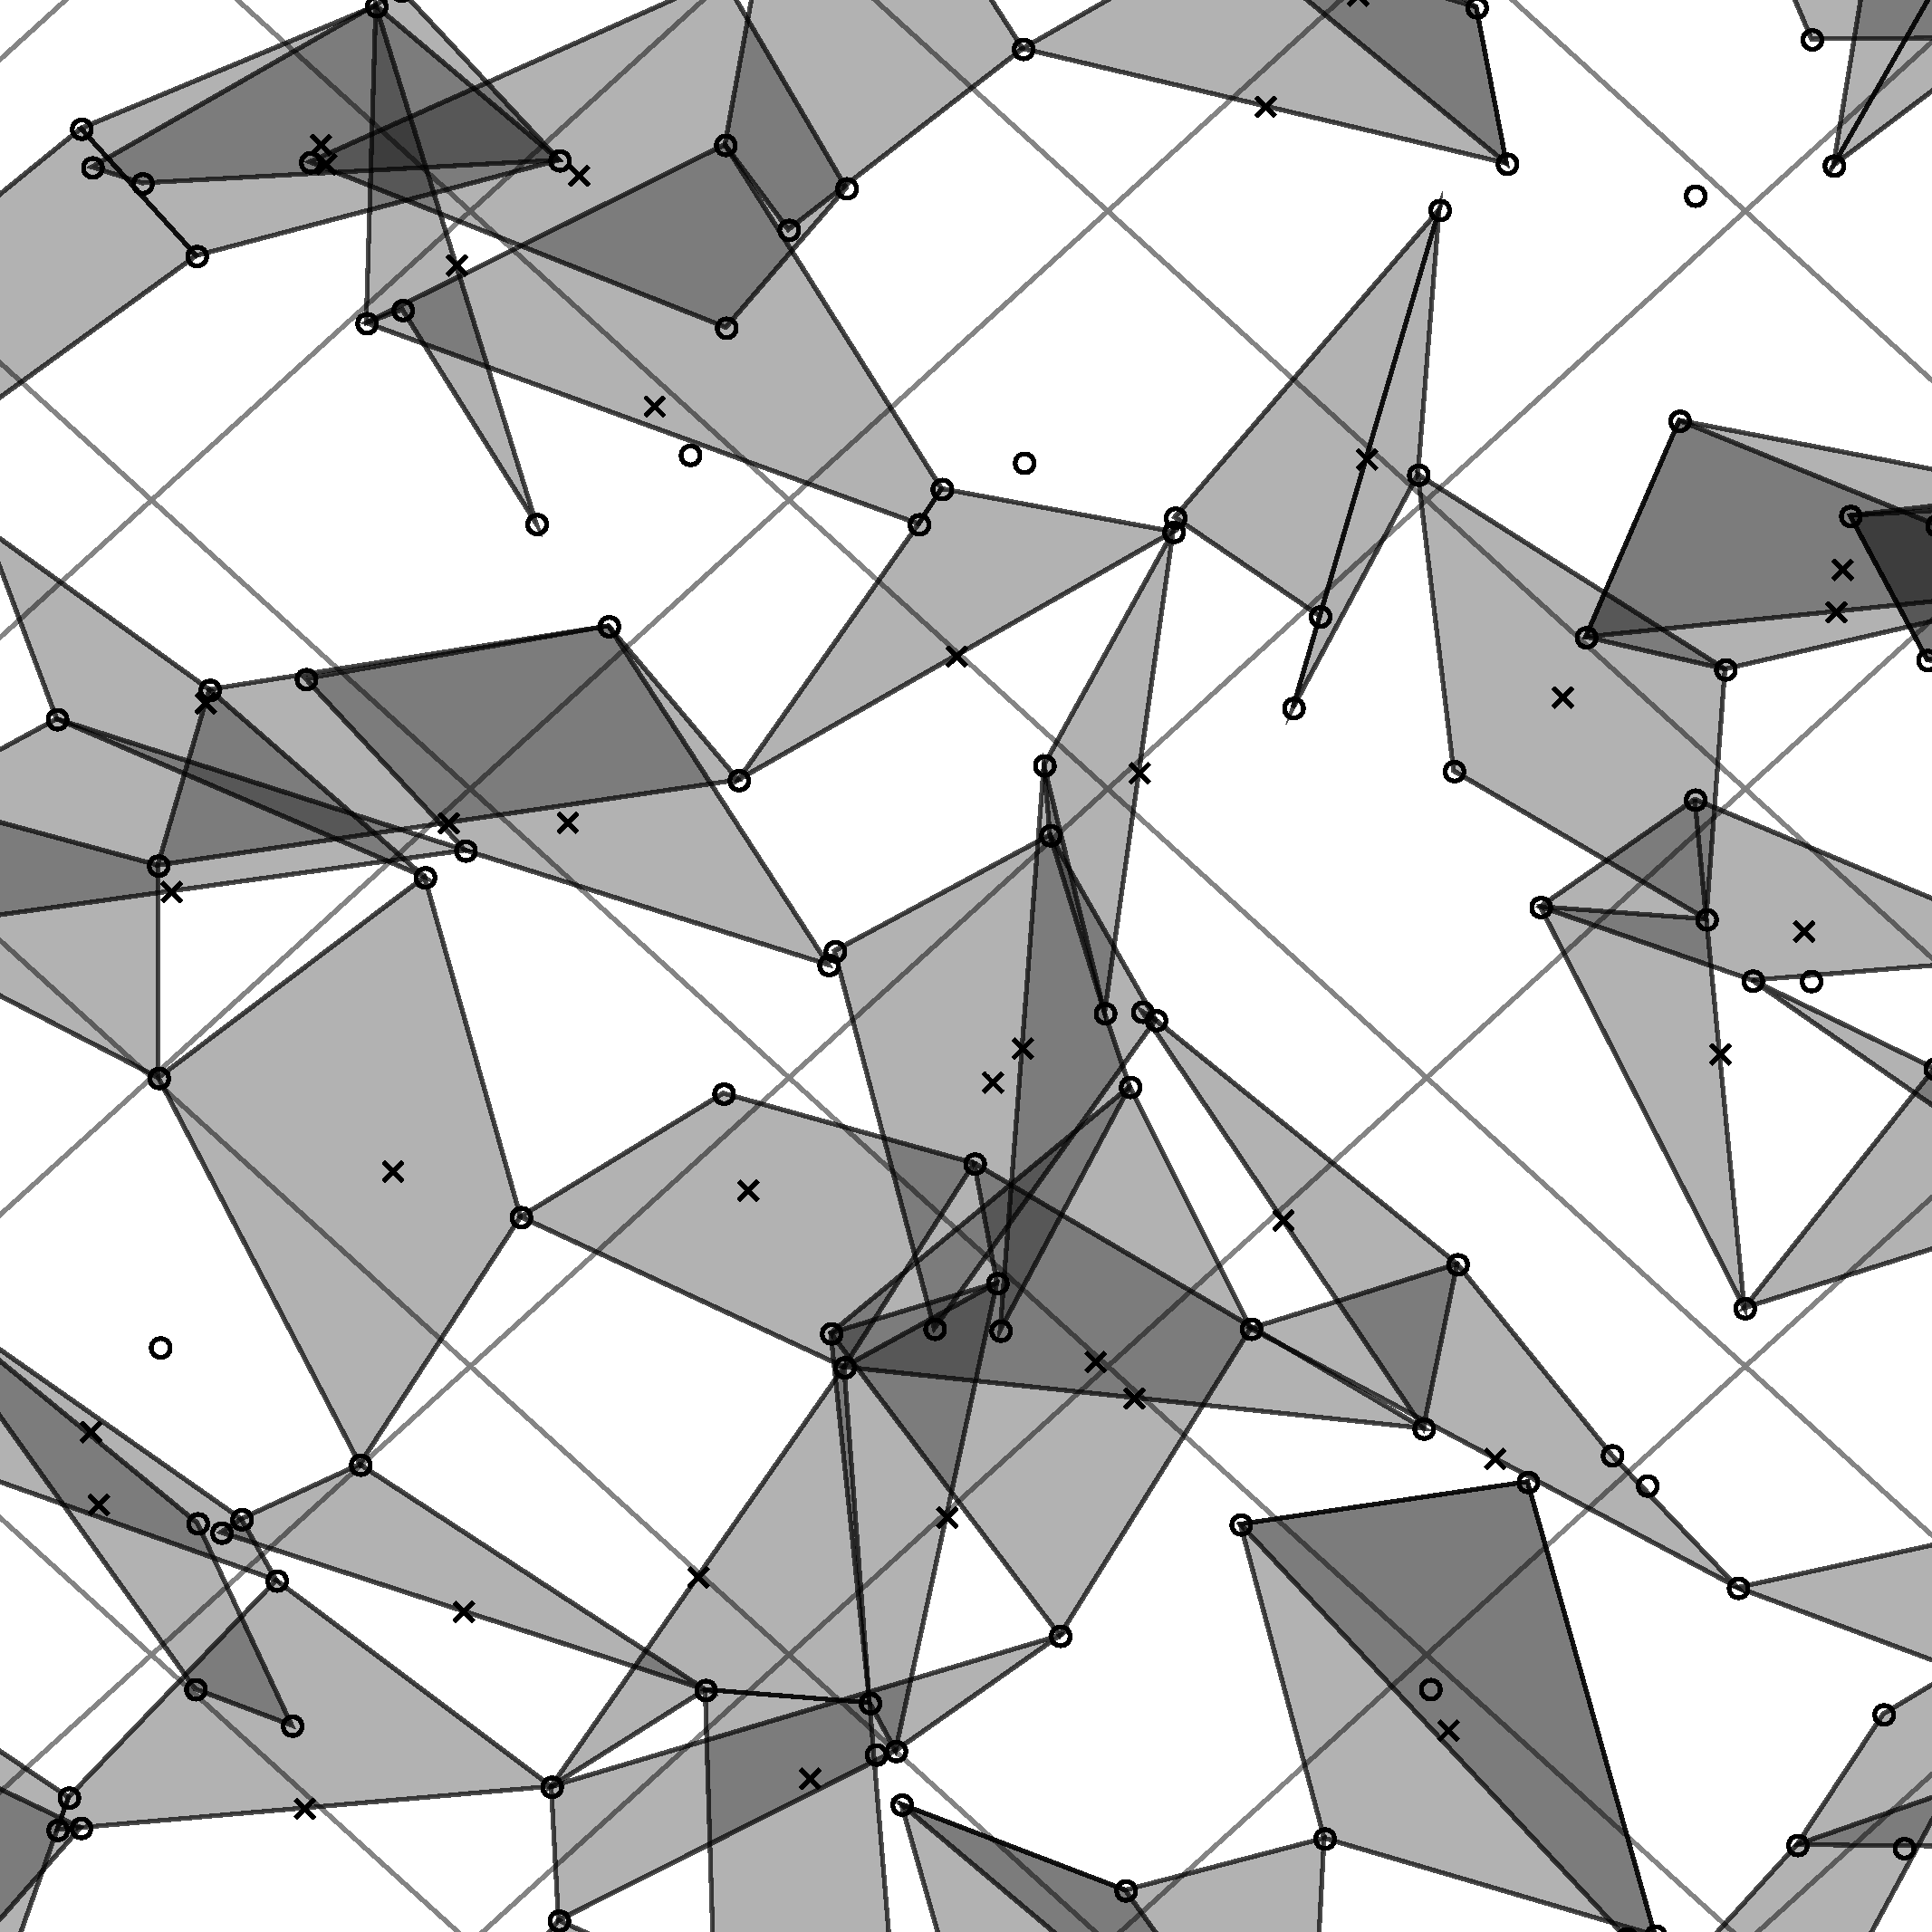
\includegraphics[height=\indfigh]{quads2b}}%
		\only<6>{\includegraphics[height=\indfigh]{quads3b}}%
	  }%
	}
    \vspace{10pt}

	\column{\cwtwo}
    \begin{minipage}[c]{1.25\textwidth}
	  \begin{itemize}
      \setlength{\itemindent}{-10pt}
	  \small
	  \item<1-> Start with USNO-B reference catalog
	  \item<2-> Place a grid over the sky
	  \item<3-> Select $n$ brightest stars in each cell
	  \item<4-> Build a geometric feature in each cell
	  \item<5-> Build \alert{another} geometric feature in each cell
	  \item<6> \ldots build $N$ geometric features in each cell
	\end{itemize}
    \end{minipage}
  \end{columns}
\end{frame}


\begin{frame}{\an: Uniform indexing}
  \begin{itemize}
  \item The resulting index has a uniform density of features
  \end{itemize}

  \begin{center}
	
\includegraphics[height=0.6\textheight]{index-1302-density}
  \end{center}
\end{frame}


\subsection{Test time}

\newcommand{\mystrut}{\rule[-1pt]{0pt}{12pt}}

\begin{frame}[plain]{\an: Test time%
	% HACK - manual changing page number.
	\ \ %
	{\small%
	\only<1>{[1/11]}%
	\only<2>{[2/11]}%
	\only<3>{[3/11]}%
	\only<4>{[4/11]}%
	\only<5>{[5/11]}%
	\only<6>{[6/11]}%
	\only<7>{[7/11]}%
	\only<8>{[8/11]}%
	\only<9>{[9/11]}%
	\only<10>{[10/11]}%
	\only<11>{[11/11]}%
	}}

  \begin{tabular}{@{}l@{\hspace{0.05\textwidth}}l@{}}
	%
	\begin{minipage}[c]{0.6\textwidth}
	\begin{itemize}
	  \small
	  \item<2-> Detect stars
	  \item<3-> Starting with the brightest stars \ldots
	  \item<4-> Build \only<1-6>{a}\only<7->{\alert{another}} geometric feature
	  \item<5-> Find matching features in the index
	  \item<6-> Check each match by looking for alignment with other stars in the index
	\end{itemize}
	\makebox[\textwidth][r]{%
	  \only<1>{\includegraphics[width=1.1\textwidth]{m88-quarter}}%
	  \only<2>{\includegraphics[width=1.1\textwidth]{m88-all-objs}}%
	  \only<3>{\includegraphics[width=1.1\textwidth]{m88-objs}}%
	  \only<4-5>{\includegraphics[width=1.1\textwidth]{m88-7-quad}}%
	  \only<6>{\includegraphics[width=1.1\textwidth]{m88-7-rg}}%
	  \only<7-8>{\includegraphics[width=1.1\textwidth]{m88-0-quad}}%
	  \only<9>{\includegraphics[width=1.1\textwidth]{m88-204-rg}}%
	  \only<10>{\includegraphics[width=1.1\textwidth]{m88-0-rg}}%
	  \only<11>{\includegraphics[width=1.1\textwidth]{m88-ann}}%
	}\\
	\end{minipage}
	%
	&
	\begin{minipage}[c]{0.35\textwidth}
	\vspace{-0.12\textheight}
	\centering
	\only<1-4>{
	  % placeholder
	  \mystrut \\
	  \rule{0pt}{0.5\textheight}\\
	  \rule{0pt}{0.5\textheight}\\
	}
	\only<5-6>{%
	  \mystrut Match \#1 \\
	  \includegraphics[height=0.5\textheight]{m88-7-zoom1}\\
	  \includegraphics[height=0.5\textheight]{m88-7-zoom4}\\
	}
	\only<7>{
	  \mystrut \\
	  \includegraphics[height=0.5\textheight]{m88-zoom1}\\
	  \rule{0.5\textheight}{0.5\textheight}\\
	}
	\only<8-9>{%
	  \mystrut Match \alert{\#1} \\
	  \includegraphics[height=0.5\textheight]{m88-204-zoom1}\\
	  \includegraphics[height=0.5\textheight]{m88-204-zoom4}\\
	}
	\only<10-11>{%
	  \mystrut Match \alert{\#2} \\
	  \includegraphics[height=0.5\textheight]{m88-0-zoom1}\\
	  \includegraphics[height=0.5\textheight]{m88-0-zoom4}\\
	}
	\end{minipage}
	\\
  \end{tabular}
\end{frame}


\section{Details}

\subsection{Checking matches}

\begin{frame}{Checking matches}
  \begin{itemize}
    \addtolength{\itemsep}{0.5ex}
    \item Feature matching generates lots of \alert{false matches}
    \item We need to \alert{decide} to accept or reject: use \alert{Bayesian decision theory}
    \item We \alert{predict} the locations of stars in the image using
      two competing models:
      \begin{itemize}
        \addtolength{\topsep}{0.5ex}
        \addtolength{\itemsep}{0.5ex}
      \item it's a true match, so we expect to find \alert{image}
        stars near \alert{index} stars (transformed according to the match)
      \item it's a false match, so image stars can be \alert{anywhere}
      \end{itemize}
    \item We really want to avoid false positives, so demand that the
      true-match model be \alert{much better} than the false-match
      model
  \end{itemize}
\end{frame}

\begin{frame}{Checking matches}
  \vspace{-10pt}
  \begin{center}
    \only<1>{\includegraphics[width=0.95\textwidth]{ror-slides-bgmodel}}
    \only<2>{\includegraphics[width=0.95\textwidth]{ror-slides-fgstars}}
    \only<3>{\includegraphics[width=0.95\textwidth]{ror-slides-fgmodel}}
    \only<4>{\includegraphics[width=0.95\textwidth]{ror-slides-bayes}}
  \end{center}
\end{frame}

\subsection{libkd}

\begin{frame}{Fast \kdtree\  implementation}
\begin{itemize}
    \addtolength{\itemsep}{0.5ex}
\item Most of our compute time is spent on \alert{two operations}:
  \begin{itemize}
    \addtolength{\itemsep}{0.5ex}
    \addtolength{\topsep}{0.5ex}
  \item Searching for \alert{nearby features} in an index
  \item Finding other stars that should be visible (when checking
    matches)
  \end{itemize}
\item Both are \alert{range-search} operations in low dimensions: perfect
  for a \kdtree
\item We created \alert{\libkd} to satisfy our needs:
  \begin{itemize}
    \addtolength{\itemsep}{0.5ex}
    \addtolength{\topsep}{0.5ex}
  \item Fast
  \item Space-efficient
  \end{itemize}
\end{itemize}
\end{frame}

\newcommand{\ftt}[1]{\tt #1}
\newcommand{\sg}[1]{{\small\color[rgb]{0.5,0.5,0.5}{#1}}}
\newcommand{\libkdmem}[3]{\multicolumn{2}{c|}{%
    \makebox[\widthof{\sg{120+}}][r]{\sg{#1+}}%
    \makebox[\widthof{\sg{52}}][r]{\sg{#2}} = %
    \makebox[\widthof{172}][r]{#3}}}
\newcommand{\compmem}[3]{\multicolumn{1}{c|}{%
    \makebox[\widthof{\sg{120+}}][r]{\sg{#1+}}%
    \makebox[\widthof{\sg{250}}][r]{\sg{#2}} = %
    \makebox[\widthof{370}][r]{#3}}}
\newcommand{\minitab}[2][l]{\begin{tabular}{#1}#2\end{tabular}}

\begin{frame}{\libkd: Performance tests}
  \setlength{\leftmargin}{-10pt}
\begin{itemize}
  \item The competition:
    \begin{itemize}
      \item \alert{Simple \kdtree s} {\small [Moore/Ostlund]}
      \item \alert{ANN} {\small [Arya \emph{et al.}]}
    \end{itemize}
  \item The test: \alert{$5$ million} points in the unit cube; \makebox[0pt][l]{nearest-neighbour} \\
    {\small (largest trees the competition could make)}
\end{itemize}
\vspace{5pt}

\commentout{
\hspace{-25pt}
\begin{minipage}[c]{\textwidth}
\begin{tabular}{|l|D{.}{}{3.0}@{\hspace{5pt}}D{.}{}{3.0}|r@{\hspace{5pt}}r|}
\hline
\multirow{3}{*}{\minitab[c]{{\bf Implementation}}} &
\multicolumn{2}{c|}{{\bf Speed}} &
\multicolumn{2}{c|}{{\bf Memory}} \\
&
\multicolumn{2}{c|}{(k q/sec)} &
\multicolumn{2}{c|}{data + tree = total (Mbytes)} \\
& \multicolumn{1}{c}{32-bit}
& \multicolumn{1}{c|}{64-bit}
& \multicolumn{1}{c}{32-bit}
& \multicolumn{1}{c|}{64-bit} \\
\hline
\ftt{simkd} &          47. &  39. & \compmem{120}{250}{370} & \compmem{120}{366}{486} \\
\ftt{ANN}   &          71. &  90. & \compmem{120}{67}{187} & \compmem{120}{101}{221} \\
\hline
\ftt{libkd-d-box}   & 127. & 144. & \libkdmem{120}{52}{172} \\
\ftt{libkd-d-split} & 231. & 284. & \libkdmem{120}{6}{126} \\
\ftt{libkd-i-split} & 242. & 311. & \libkdmem{ 60}{4}{64} \\
\ftt{libkd-s-split} & 328. & 386. & \libkdmem{ 30}{3}{33} \\
\hline
\end{tabular}
\end{minipage}
}

\end{frame}

\begin{frame}{\libkd: Memory required (smaller is better)}
\begin{center}
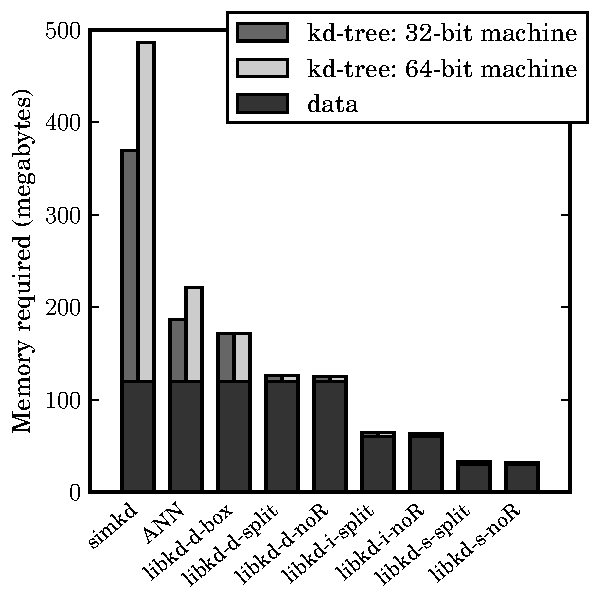
\includegraphics[height=0.85\textheight]{kd-bar-mem}
\end{center}
\end{frame}

\begin{frame}{\libkd: Speed (bigger is better)}
\begin{center}
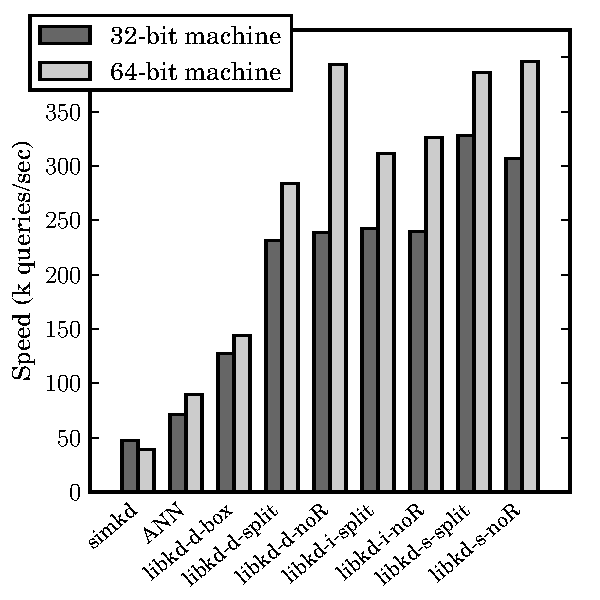
\includegraphics[height=0.85\textheight]{kd-bar-speed}
\end{center}
\end{frame}



\section{Results}

\subsection{SDSS}

\begin{frame}{\an: Performance}
  \begin{itemize}
    \addtolength{\itemsep}{0.5ex}
  \item Took $330,000$ images from the Sloan Digital Sky Survey (SDSS) rated ``acceptable'' or better
  \item Correctly recognized over \alert{$99.95~\%$}
  \item With some fancy footwork, recognized \alert{$100~\%$} of the $183,359$ images rated ``excellent''
  \item \alert{No false positives}: we are either correct or give no-answer
  \item Most images take less than \alert{$1$ second} of CPU time
    \\ \small (given strong hints about the image scale)
  \end{itemize}
\end{frame}

\begin{frame}{\an: Performance}
  \vspace{-10pt}
  \begin{center}
    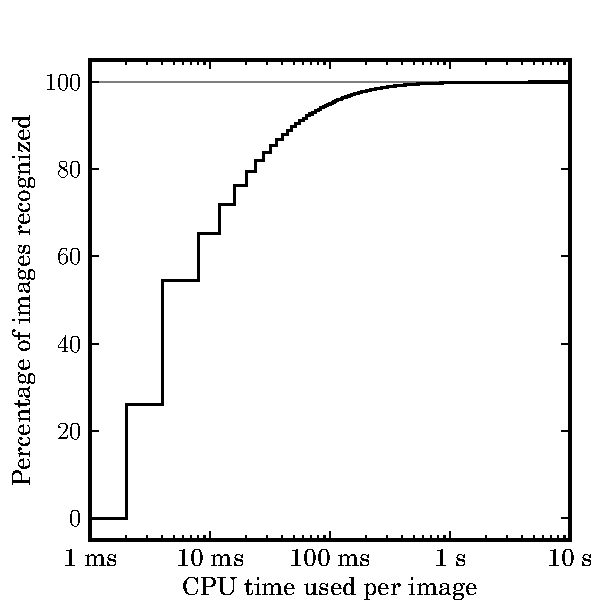
\includegraphics[height=0.9 \textheight]{sdss-er-cputime}
  \end{center}
\end{frame}

\begin{frame}{\an: Performance --- scale hints}
  \vspace{-10pt}
  \begin{center}
    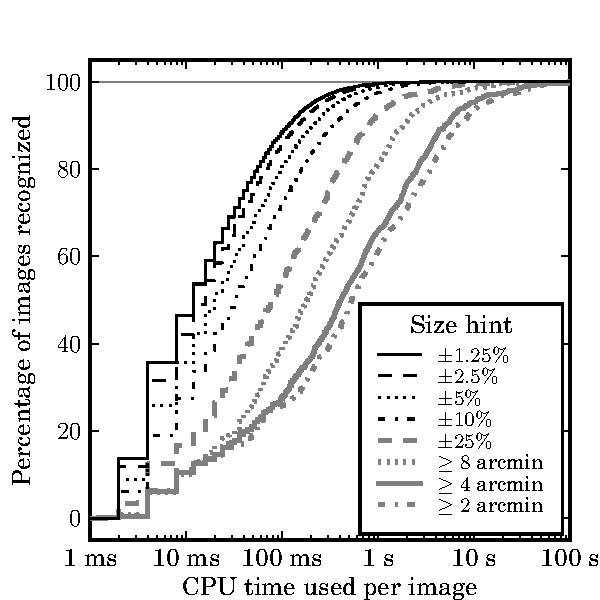
\includegraphics[height=0.9 \textheight]{sdss-sizehints-time}
  \end{center}
\end{frame}

\begin{frame}{\an: Performance --- triangles \& quintuples}
  \vspace{-10pt}
  \begin{center}
    \only<1>{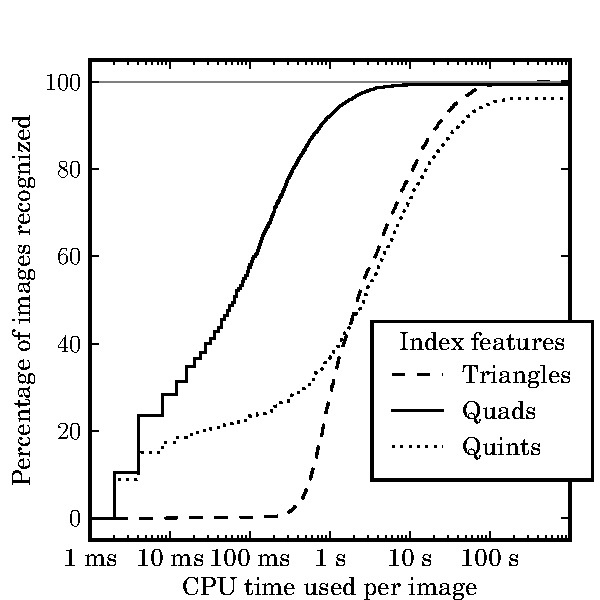
\includegraphics[height=0.9 \textheight]{sdss-triquint-time}}%
    \only<2>{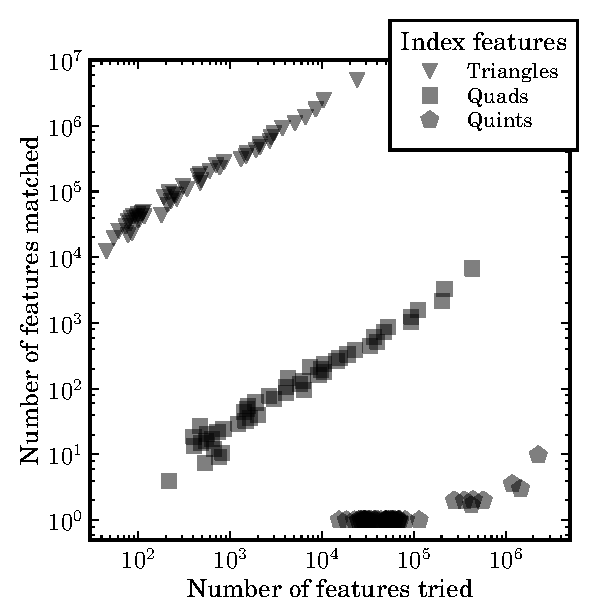
\includegraphics[height=0.9 \textheight]{sdss-triquint-ntrynmatch}}%
  \end{center}
\end{frame}


\subsection{GALEX, HST}

\begin{frame}{\an: Other data sets}
  We get excellent results on SDSS images.
  \vspace{12pt}

  We've also tested:
  \begin{itemize}
    \addtolength{\itemsep}{0.5ex}
  \item images from \alert{GALEX}, a space telescope that measures
    ultraviolet (UV): \alert{$99.7\%$} recognition rate for near-UV
  \item images from the \alert{Hubble Space Telescope}'s Advanced
    Camera for Surveys --- with a custom-built index ---
    \alert{$100\%$} success on a tiny sample of $191$ images
  \end{itemize}
\end{frame}


\subsection{Users}

\begin{frame}{\an: Users}
  \begin{itemize}
    \addtolength{\itemsep}{0.5ex}
  \item Open-source code, web version, and Flickr robot \\
    (thousands of testers; running since 2007 April)
  \item Digital archives: the DeepSky project is reprocessing
    Palomar-QUEST data: \alert{\mbox{$14$ million}} images so far
  \item Photographic archives: the DASCH project is scanning \alert{$500,\!000$
    photographic glass plates} (taken 1880 to 1985) from the Harvard
    archives
  \item Amateur astronomers: the Royal Observatory Greenwich are
    adding \alert{astro-tags} to their Astronomy Photographer of the Year
    competition
  \end{itemize}
  \vspace{10pt}

  We've been featured in: Nature news, IEEE Spectrum, Toronto Star, CBC.ca, Flickr Blog, Slashdot, \ldots
  
\end{frame}



\section{Conclusion}

\begin{frame}[label=conclusion]{Conclusion}
  \begin{itemize}
    \addtolength{\itemsep}{0.5ex}
  \item \an\  can automatically recognize a wide variety of astronomical images
  \item Makes a lot of ``\alert{lost data}'' available to astronomers
    \begin{itemize}
    \item Useful for \alert{time-domain} work: rapid cadence from
      amateur astronomers and long time baselines from historical
      photographs
    \end{itemize}
  \item Important for \alert{verifying} or \alert{creating} meta-data
    in the Virtual Observatory
  \item \an\ is a computer vision system that \alert{works}, in one domain of images
    %\begin{itemize}
    %  \item Part of the renaissance of geometry in computer vision?
    %\end{itemize}
  \end{itemize}
\end{frame}

\begin{frame}{Thanks!}

\alert{Time for questions and discussion!}

\vspace{1em}
My great collaborators:
\begin{itemize}
  \item Sam Roweis (Toronto / Google)
  \item David~W.~Hogg (NYU)
  \item Keir Mierle (Google)
  \item Christopher Stumm (Microsoft)
  \item Jon Barron (Berkeley)
  \item Michael Blanton (NYU)
\end{itemize}
\end{frame}

%\end{comment}

\begin{frame}{How much of this is your work?}
  \includegraphics[height=0.9\textheight]{svn}
\end{frame}

\begin{frame}{False positive example}
\vspace{-8pt}
\begin{center}
\framebox{%
\only<1>{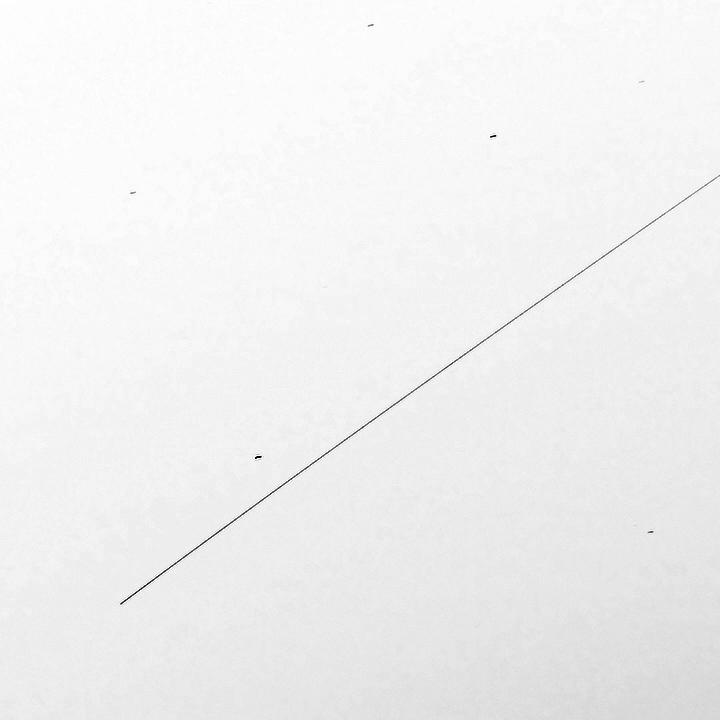
\includegraphics[height=0.87\textheight]{iss-inv}}%
\only<2>{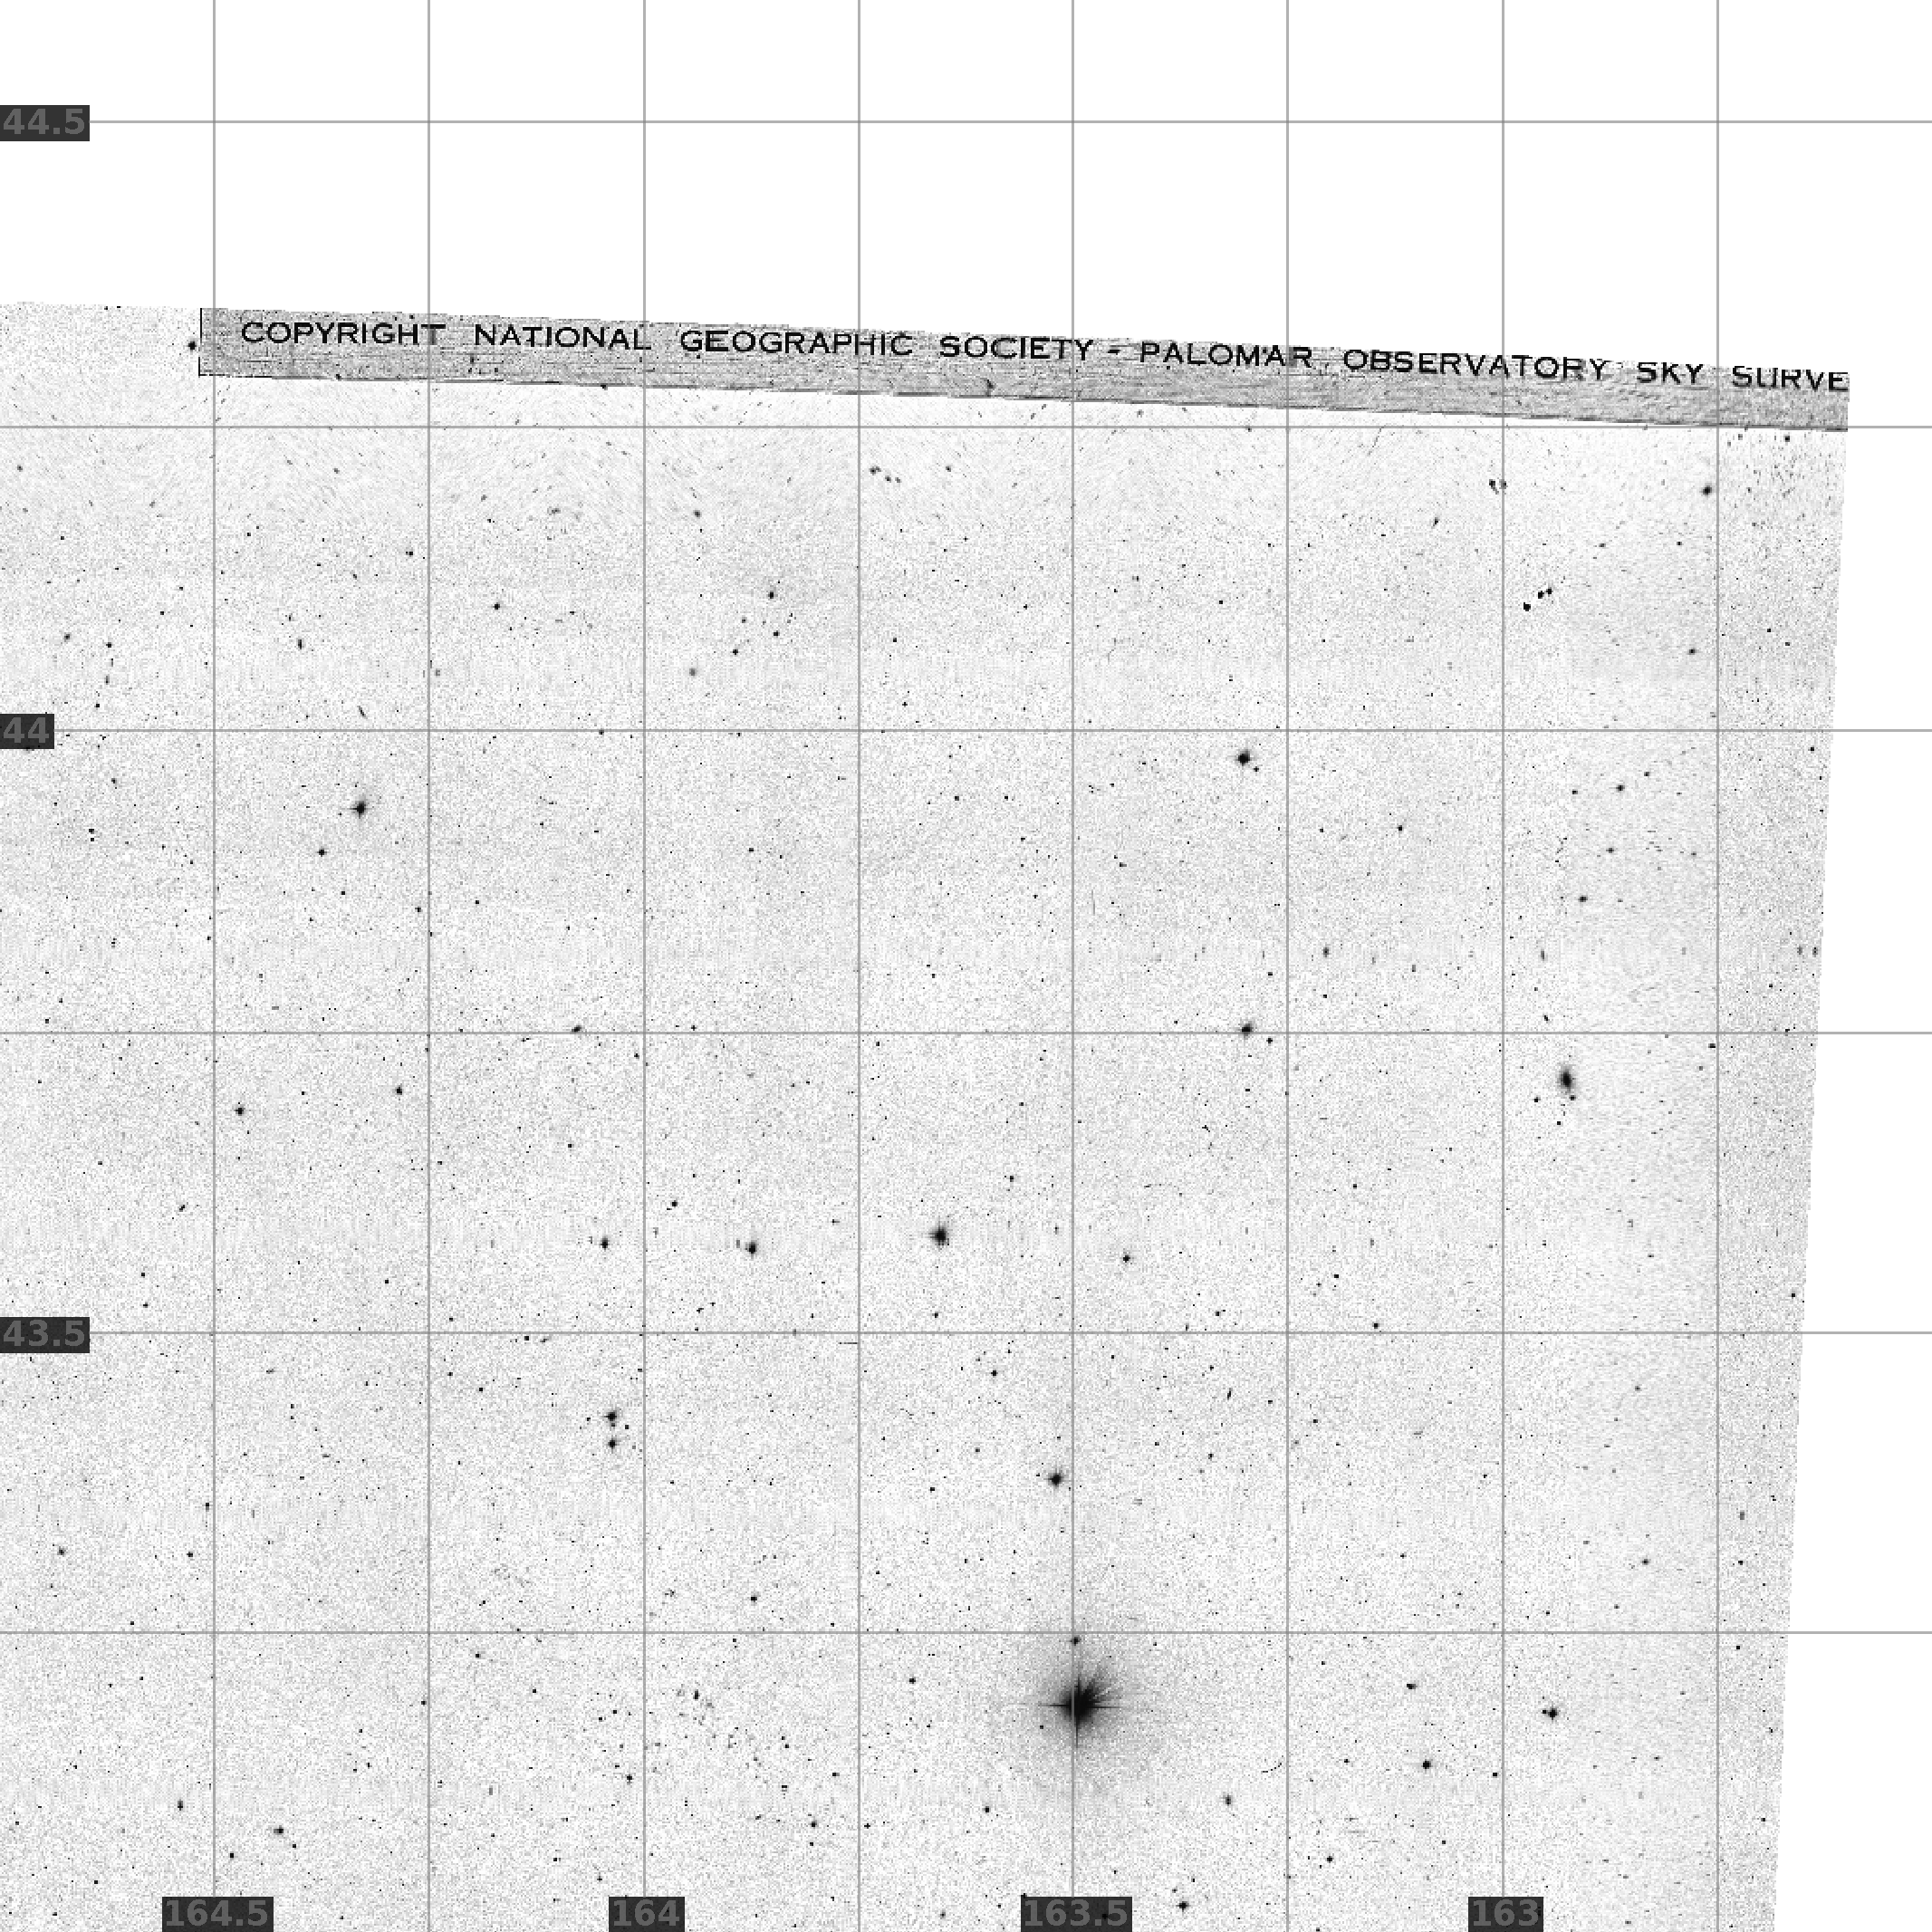
\includegraphics[height=0.87\textheight]{usnob-iss}}%
\only<3>{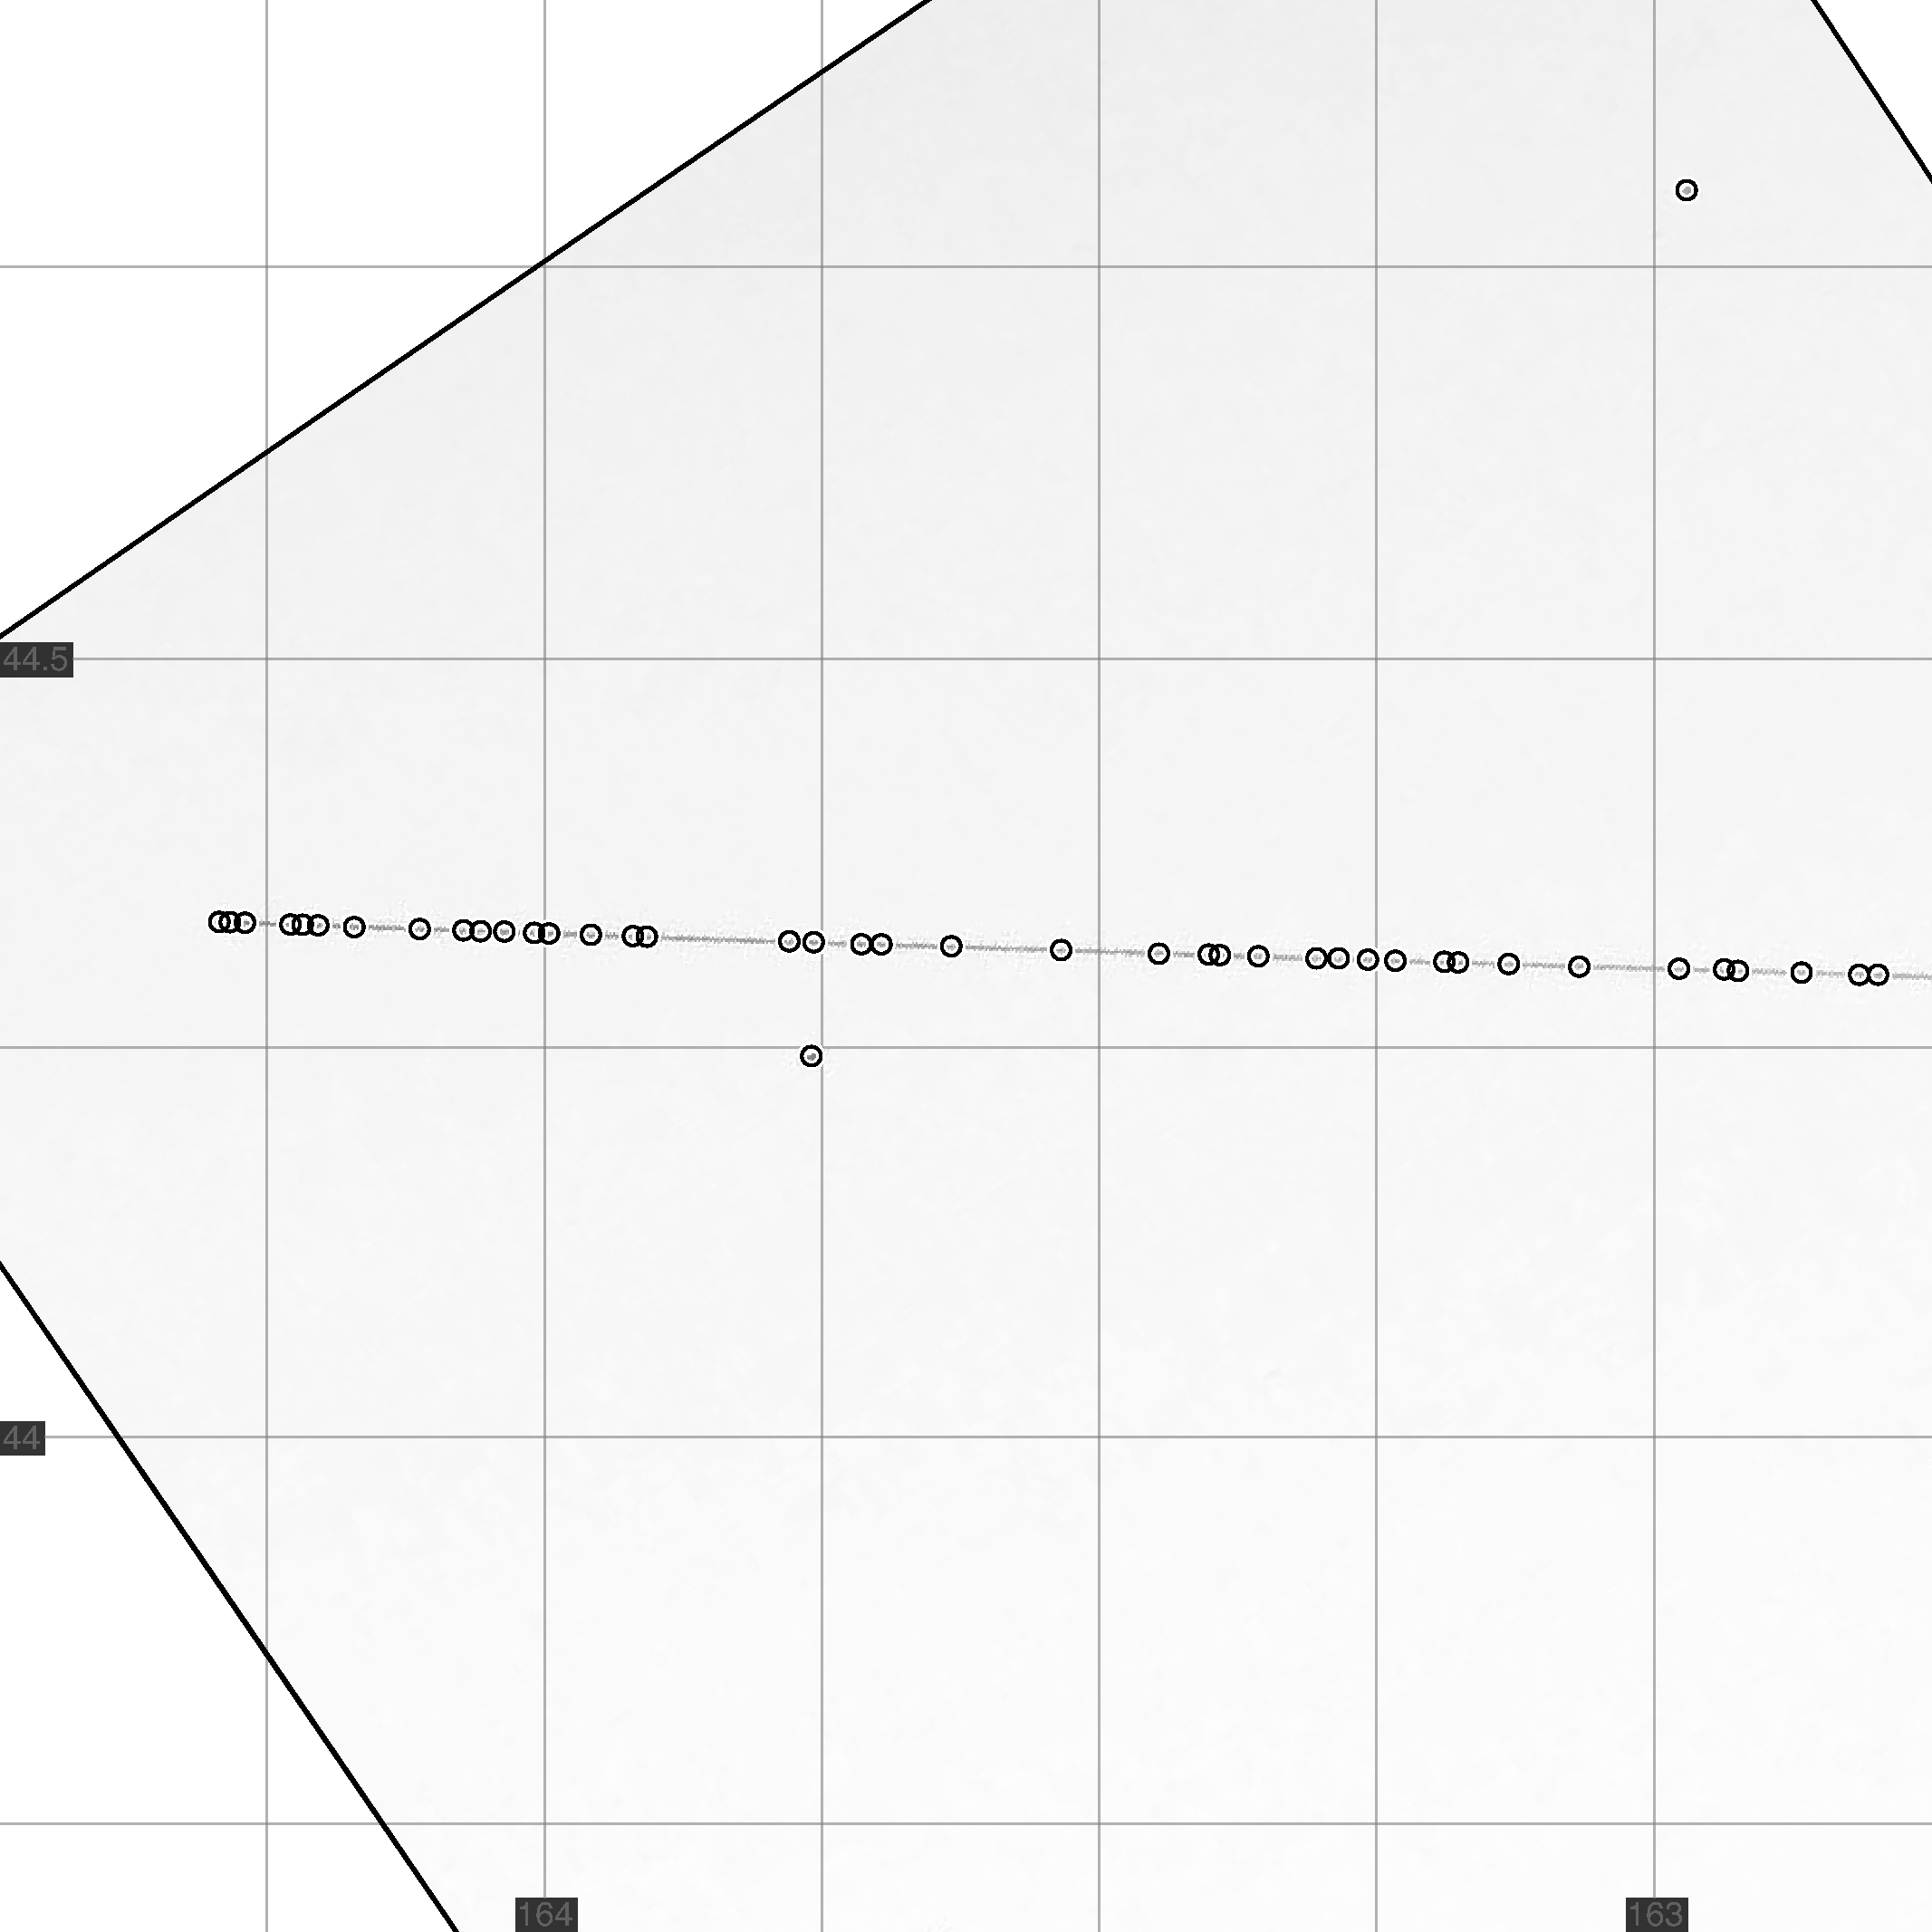
\includegraphics[height=0.87\textheight]{iss-img-xy}}%
\only<4>{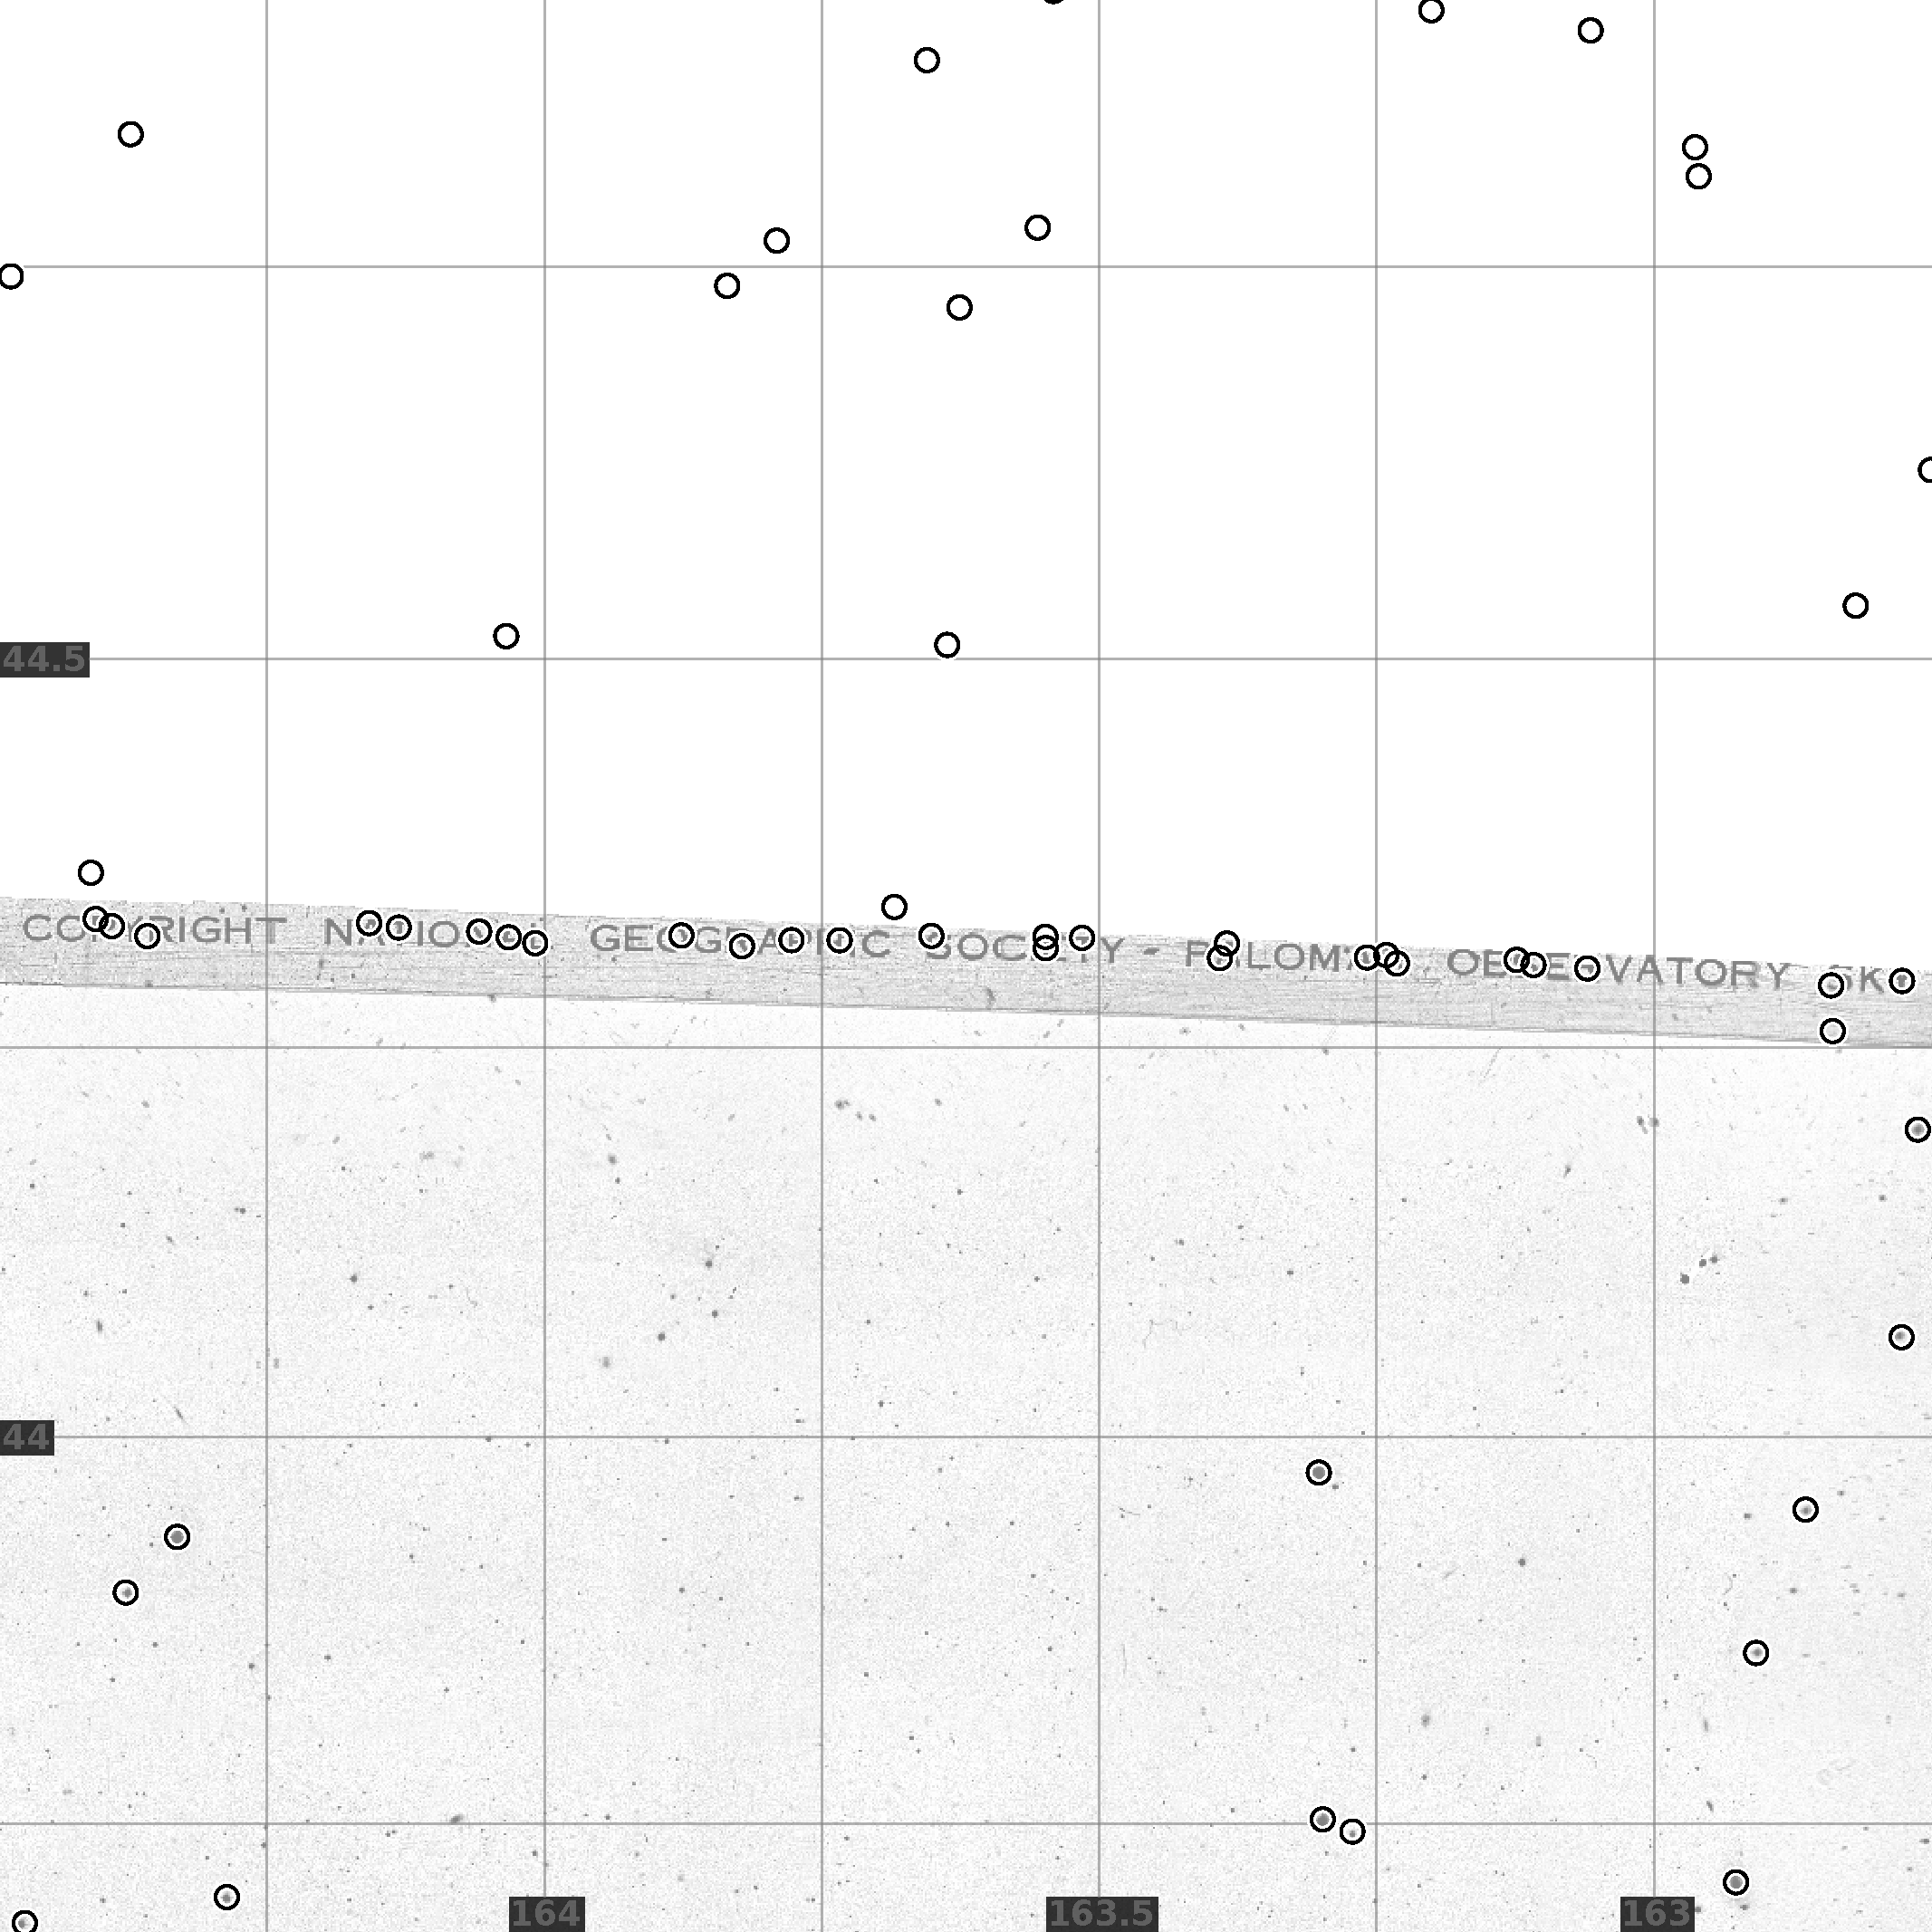
\includegraphics[height=0.87\textheight]{iss-usnob-xy}}%
}
\end{center}
\end{frame}

\section[]{Comet Holmes: Crowd-sourced astronomy}

\begin{frame}{Comet Holmes: Crowd-sourced astronomy}
  \begin{itemize}
  \item Did a Yahoo Image Search for ``Comet Holmes''
  \item Fed the first $1000$ images into \an
  \item $500$ were recognized
  \end{itemize}
\end{frame}

\begin{frame}{Comet Holmes: Crowd-sourced astronomy}
  \begin{center}
  \begin{tabular}{cc}
    \includegraphics[height=0.33\textheight]{holmes1}&
    \includegraphics[height=0.33\textheight]{holmes3}\\
    \includegraphics[height=0.33\textheight]{holmes2}&
    \includegraphics[height=0.33\textheight]{holmes4}
  \end{tabular}
  \\
  {
    \Tiny
    TL: \url{http://gaussling.files.wordpress.com/2007/11/comet-holmes.jpg}
    \\
    TR: \url{http://www.clarkvision.com/galleries/images.astrophoto-1/web/comet.holmes.c10.31.2007.36s2.d-c800.jpg}
    \\
    BL: \url{http://astro.uchicago.edu/yerkes/pics/Comet\%20Holmes\%201028a.JPG}
    \\
    BR: \url{http://spaceweather.com/comets/holmes/13nov07/Jay-Edwards-Comet_holmes_20071110_55MM_1194912215.jpg}
    \\
  }
  \end{center}
\end{frame}

\begin{frame}{Comet Holmes: Pixel density}
  \begin{center}
    \includegraphics[height=0.9\textheight]{holmes-density-allsky}
  \end{center}
\end{frame}

\begin{frame}{Comet Holmes: Pixel density (zoom)}
  \begin{center}
    \includegraphics[height=0.9\textheight]{holmes-density}
  \end{center}
\end{frame}

\begin{frame}{Comet Holmes: Pixel density and true path}
    \begin{center}
    \includegraphics[height=0.9\textheight]{holmes-density-path}
  \end{center}
\end{frame}

\begin{frame}{Comet Holmes: Timestamps from EXIF}
  \vspace{-1ex}
  \begin{center}
    \includegraphics[height=0.9\textheight]{holmes-timestamps}
  \end{center}
\end{frame}

\begin{frame}{Comet Holmes: Crowd-sourced astronomy (5)}
  \begin{itemize}
    \item With just the search phrase ``\alert{Comet Holmes}'', we can
      get the comet's path through the sky, with timestamps
    \item From this, you can determine the \alert{orbital elements}
      that describe its 3-d orbit [work in progress]
    \item \ldots and all this without even locating the comet in the
      images!
  \end{itemize}
\end{frame}


\end{document}


